% ---
% titre: Conversion d'unités
% theme: GM
% chapitre: Lignes et surfaces
% sous_chapitre: Polygones
% niveau: [9e]
% type: EVAL
% tags: [c-calcul-aires, p-question-TS]
% difficulte: 1
% corrige: true
% ---

\newpage
\question[15]
Calcule le périmètre et l'aire des figures suivantes. Pour chaque question, note le nom de la figure, la formule générale, ainsi que tes calculs. N'oublie pas l'unité!

\begin{parts}

\vspace{20pt}\part[2]\,

\begin{minipage}{0.45\linewidth}
\begin{center}
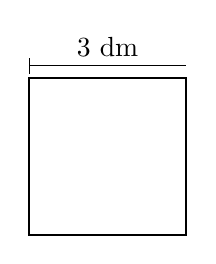
\begin{tikzpicture}[scale=1]
    \draw[thick] (0,0) rectangle (2,2);
    \draw[-|,|-] (0,2.15) -- (2,2.15) node[midway,above]{3 dm};
\end{tikzpicture}
\end{center}
\end{minipage}
\hfill
\begin{minipage}{0.5\linewidth}
{\footnotesize\raggedleft Espace pour ta démarche et tes calculs\par}
\begin{solutionorgrid}[100pt]
P = $4\cdot 3 = 12\,[\text{dm}]$ \hfill \textbf{(1pt)}\\[6pt]
A = $3^2 = 9\,[\text{dm}^2]$ \hfill \textbf{(1pt)}
\end{solutionorgrid}
\end{minipage}

\vspace{20pt}\part[2]\,

\begin{minipage}{0.45\linewidth}
\begin{center}
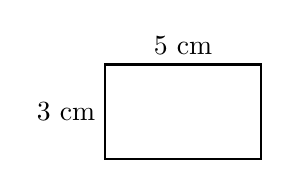
\begin{tikzpicture}[scale=0.6]
    \draw[thick] (0,0) rectangle (3.3,2);
    \node[above] at (1.65,2) {5 cm};
    \node[left] at (0,1) {3 cm};
\end{tikzpicture}
\end{center}
\end{minipage}
\hfill
\begin{minipage}{0.5\linewidth}
{\footnotesize\raggedleft Espace pour ta démarche et tes calculs\par}
\begin{solutionorgrid}[100pt]
P = $2\cdot(5+3) = 16\,[\text{cm}]$ \hfill \textbf{(1pt)}\\[6pt]
A = $5\cdot 3 = 15\,[\text{cm}^2]$ \hfill \textbf{(1pt)}
\end{solutionorgrid}
\end{minipage}

\vspace{20pt}\part[3]\,

\begin{minipage}{0.45\linewidth}
\begin{center}
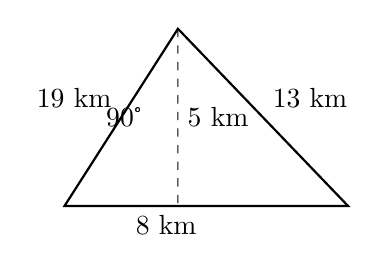
\begin{tikzpicture}[scale=0.45]
    \coordinate (A) at (0,0);
    \coordinate (B) at (8,0);
    \coordinate (C) at (3.2,5);
    \draw[thick] (A) -- (B) -- (C) -- cycle;
    \draw[dashed] (C) -- (3.2,0);
    \node[right] at (0.9,2.5) {90°};
    \node[below left] at (4,0) {8 km};
    \node[right] at (3.2,2.5) {5 km};
    \node[above left] at (1.6,2.5) {19 km};
    \node[above right] at (5.6,2.5) {13 km};
\end{tikzpicture}
\end{center}
\end{minipage}
\hfill
\begin{minipage}{0.5\linewidth}
{\footnotesize\raggedleft Espace pour ta démarche et tes calculs\par}
\begin{solutionorgrid}[100pt]
P = $19+13+8 = 40\,[\text{km}]$ \hfill \textbf{(1pt)}\\[6pt]
A = $\dfrac{8\cdot 5}{2} = 20\,[\text{km}^2]$ \hfill \textbf{(2pt)}
\end{solutionorgrid}
\end{minipage}

\vspace{20pt}\part[3]\,

\begin{minipage}{0.45\linewidth}
\begin{center}
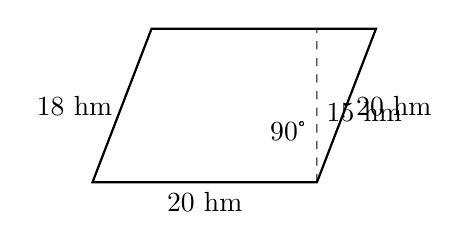
\begin{tikzpicture}[scale=0.3]
    \coordinate (A) at (0,0);
    \coordinate (B) at (9.5,0);
    \coordinate (C) at (12,6.5);
    \coordinate (D) at (2.5,6.5);
    \draw[thick] (A) -- (B) -- (C) -- (D) -- cycle;
    \draw[dashed] (B) -- (9.5,6.5);
    \node[below left] at (9.5,3) {90°};
    \node[below] at (4.75,0) {20 hm};
    \node[right] at (9.5,3) {15 hm};
    \node[left] at (1.25,3.25) {18 hm};
    \node[right] at (10.75,3.25) {20 hm};
\end{tikzpicture}
\end{center}
\end{minipage}
\hfill
\begin{minipage}{0.5\linewidth}
{\footnotesize\raggedleft Espace pour ta démarche et tes calculs\par}
\begin{solutionorgrid}[100pt]
P = $2\cdot(18+20) = 76\,[\text{hm}]$ \hfill \textbf{(1pt)}\\[6pt]
A = $20\cdot 15 = 300\,[\text{hm}^2]$ \hfill \textbf{(2pt)}
\end{solutionorgrid}
\end{minipage}

\newpage}\part[2]\,

\begin{minipage}{0.45\linewidth}
\begin{center}
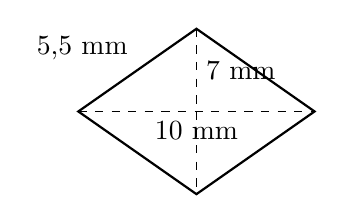
\begin{tikzpicture}[scale=0.3]
    \coordinate (A) at (0,0);
    \coordinate (B) at (5,3.5);
    \coordinate (C) at (10,0);
    \coordinate (D) at (5,-3.5);
    \draw[thick] (A) -- (B) -- (C) -- (D) -- cycle;
    \draw[dashed] (A) -- (C);
    \draw[dashed] (B) -- (D);
    \node[above left] at (2.5,1.75) {5,5 mm};
    \node[below] at (5,0) {10 mm};
    \node[right] at (5,1.75) {7 mm};
\end{tikzpicture}
\end{center}
\end{minipage}
\hfill
\begin{minipage}{0.5\linewidth}
{\footnotesize\raggedleft Espace pour ta démarche et tes calculs\par}
\begin{solutionorgrid}[100pt]
P = $4\cdot 5,5 = 22\,[\text{mm}]$ \hfill \textbf{(1pt)}\\[6pt]
A = $\dfrac{10\cdot 7}{2} = 35\,[\text{mm}^2]$ \hfill \textbf{(1pt)}
\end{solutionorgrid}
\end{minipage}

\vspace{20pt}\part[3]\,

\begin{minipage}{0.45\linewidth}
\begin{center}
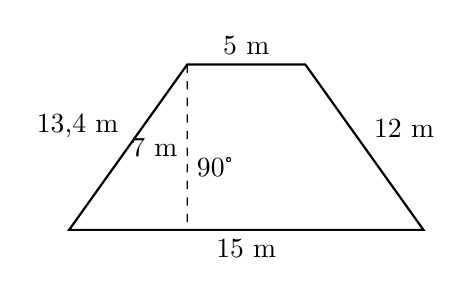
\begin{tikzpicture}[scale=0.3]
    \coordinate (A) at (0,0);
    \coordinate (B) at (5,7);
    \coordinate (C) at (10,7);
    \coordinate (D) at (15,0);
    \draw[thick] (A) -- (B) -- (C) -- (D) -- cycle;
    \draw[dashed] (B) -- (5,0);
    \node[below right] at (5,3.5) {90°};
    \node[above] at (7.5,7) {5 m};
    \node[below] at (7.5,0) {15 m};
    \node[left] at (5,3.5) {7 m};
    \node[above left] at (2.5,3.5) {13,4 m};
    \node[above right] at (12.5,3.5) {12 m};
\end{tikzpicture}
\end{center}
\end{minipage}
\hfill
\begin{minipage}{0.5\linewidth}
{\footnotesize\raggedleft Espace pour ta démarche et tes calculs\par}
\begin{solutionorgrid}[100pt]
P = $15+5+13,4+12 = 45,4\,[\text{m}]$ \hfill \textbf{(1pt)}\\[6pt]
A = $\dfrac{(15+5)}{2}\cdot 7 = 70\,[\text{m}^2]$ \hfill \textbf{(2pt)}
\end{solutionorgrid}
\end{minipage}

\end{parts}